% !TeX spellcheck = ru_RU
% !TEX root = vkr.tex

\subsection{Поддержка обобщенных атомарных операций}
Когда речь идёт о библиотеке обобщенных вычислений на GPGPU, проблема использования произвольных атомарных операций встает весьма остро. Их отсутствие существенно ограничивает спектр доступных алгоритмов, в том числе необходимых в задачах линейной алгебры. Стандарт OpenCL позволяет использовать некоторый набор атомарных функций над небольшим множество примитивных типов, однако для реализации обобщенных алгоритмов этого оказывается недостаточно. К сожалению, общепринятого решения этой проблеме найти не удалось. Среди аналогичных инструментов только ILGPU имеет возможность конструировать и использовать произвольные атомарные операции на основе неатомарных. Для этого в библиотеке есть статический метод \verb|MakeAtomic|, контракт которого приведен в листинге~\ref{lst:makeAtomic}. В качестве реализации используется цикл активного ожидания.

\begin{lstlisting}[caption= Контракт метода MakeAtomic, language=C, frame=single, label={lst:makeAtomic}]
public T MakeAtomic<T, TOperation, TCompareExchangeOperation>(
    ref T target,
    T value,
    TOperation operation,
    TCompareExchangeOperation compareExchangeOperation)
\end{lstlisting}

% \footnote{Один из способов расширить множество доступных атомарных операций: \url{https://stackoverflow.com/a/31865819/17106499}. Дата посещения 09.03.2022}
Существует и альтернативный способ расширить множество доступных для использования атомарных операций. Этот способ использует знание о том, что устройства, реализующие стандарт OpenCL, обеспечивают поддержку атомарных операций над 64-битными целочисленным типом \text{long}, в то время как поддержка других 64-битных типов (например, \text{double}) не гарантируется. Это ограничение можно обойти за счет использования union структуры, объединяющей любой 64-битный тип с типом \text{long}\footnote{Ссылка на предлагаемое решение: \url{https://stackoverflow.com/questions/31863587/atomic-operations-with-double-opencl/31865819#31865819}. (Дата посещение: 27.05.2022)}. Очевидным недостатком такого решения является то, что оно подходит только для типов размером 64 бита.

В данной работе поддержка произвольных атомарных операций выполнена за счет генерации функций, реализующих спинлок. Для этого язык ядра был расширен функцией \verb|atomic| с сигнатурой, приведенной в листинге~\ref{lst:atomic}. Несмотря на то, что это обыкновенная функция языка F\#, её применение внутри кода ядра ограниченно. Так, существуют ограничения на используемые в качестве первого параметра выражения --- это должна быть либо переменная, либо обращение к массиву по индексу, а также ограничены возможности ее частичного применения. Обработкой этой функции занимается соответсвующий шаг на этапе преобразования синтаксического дерева (как изображено на рисунке~\ref{fig:transl2}), который генерирует спинлок и заменяет вызов функции \verb|atomic| на вызов функции, реализующей этот спинлок. Кроме того, он преобразует код ядра таким образом, чтобы обеспечить возможность выделения памяти под мьютексы --- для каждого массива, доступ к которому необходимо ограничить взаимным исключением, выделяется дополнительный массив 32-битных целых чисел соответствующей длины, заполненный нулями. Таким образом, например, код ядра на языке F\#, приведенный в листинге~\ref{lst:atomicKernel}, преобразуется в код на языке OpenCL C, приведенный в листинге~\ref{lst:generatedAtomic}. Стоит также отметить, что в случае, когда вызов функции \text{atomic} можно преобразовать в вызов нативной атомарной функции OpenCL, спинлок не генерируется.

\begin{figure}[h!]
\centering
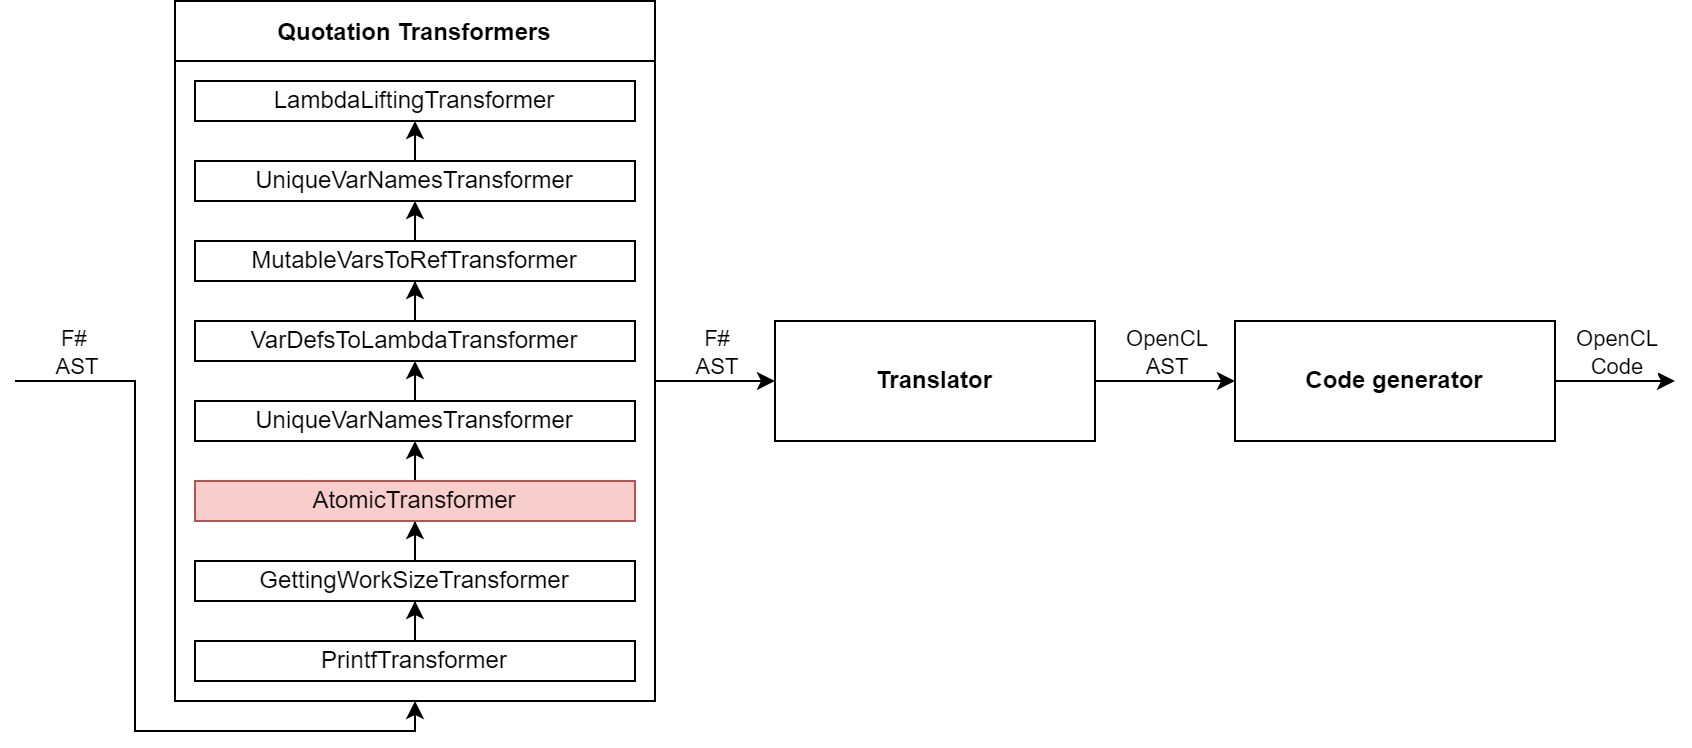
\includegraphics[scale=0.25]{pictures/Modified.png}
\caption{Этап преобразования функции atomic в модели трансляции}
\label{fig:transl2}
\end{figure}

\newpage

\begin{lstlisting}[caption=Сигнатура функции atomic, language=Caml, frame=single, label={lst:atomic}]
val atomic : ('a -> 'b) -> ('a -> 'b)
\end{lstlisting}

\begin{lstlisting}[caption=Код OpenCL ядра на языке F\#, language=Caml, frame=single, label={lst:atomicKernel}]
<@
    fun (range: Range1D) (buf: ClArray<int>) ->
        atomic (fun x -> x + 1) buf.[0] |> ignore
@>
\end{lstlisting}

\begin{lstlisting}[caption=Код OpenCL ядра после трансляции в C, language=C, frame=single, label={lst:generatedAtomic}]
#pragma OPENCL EXTENSION cl_khr_global_int32_base_atomics: enable
#pragma OPENCL EXTENSION cl_khr_local_int32_base_atomics: enable

int baseFunc(private int x)
{
    return (x + 1);
}

int atomicFunc(__local int* localAccMutex, __local int* x) {
    int oldValue;
    bool flag = 1;
    while (flag) {
        int old = atom_xchg(&localAccMutex[0], 1);
        if (old == 0) {
            oldValue = *x;
            *x = baseFunc(*x);
            atom_xchg(&localAccMutex[0], 0);
            flag = 0;
        };
        barrier(CLK_LOCAL_MEM_FENCE);
    };
    return oldValue;
}
\end{lstlisting}

% Первые тесты этого решения показали и его основной недостаток: спинлок плохо подходит для использования в программах для GPGPU. Работоспособность текущей реализации сильно зависит от платформы, на которой исполняется код, поэтому имеет смысл сделать транслятор машинозависимым. Однако, как показывает практика, даже это не дает гарантий, что генерируемый код будет вести себя единообразно на всех возможных устройствах.

Предложенное решение имеет и свои недостатки. Так, например, при использовании сгенерированной атомарной функции выделяется дополнительная память под массив мьютексов, что может быть неочевидно для пользователя. Кроме того, решение обладает низкой переносимостью из-за особенностей реализации OpenCL на каждом конкретном устройстве --- как показывает практика, нет гарантий того, что генерируемый код будет вести себя единообразно на всех возможных устройствах.

\subsection{Поддержка трансфера пользовательских типов данных}
В задачах, связанных с обработкой графов, метки ребер могут иметь произвольный тип. В связи с этим стандарт GraphBLAS не налагает ограничений на тип элементов матрицы. Эталонная реализация \\ GraphBLAS на CPU --- SuiteSparse --- позволяет использовать любою структуру фиксированного размера. Поэтому возникает необходимость обеспечить поддержку использования пользовательских структур данных. Кроме структур, интерес вызывает возможность использования размеченных объединений в ядрах OpenCL. Так, с помощью типа данных \verb|Option| естественно выражается наличие в графе ребра с некоторым весом или его отсутствие. Использование типа \verb|Option| для реализации GraphBLAS может решить проблему <<явных нулей>>\footnote{Обсуждение необходимости фильтровать явные нули: \url{https://github.com/GraphBLAS/LAGraph/issues/28}. Дата обращения: 09.03.2022}, которая вызывает дискуссии в сообществе до сих пор.

Несмотря на то, что транслятор уже умел транслировать некоторые пользовательские типы данных (кортежи, структуры, размеченные объединения), трансфер данных таких типов из управляемой памяти в видеопамять и наоборот реализован не был. Среди аналогичных инструментов лишь ILGPU и FSCL поддерживают использование пользовательских типов данных. Рантайм библиотеки ILGPU способен оперировать любыми типами, которые удовлетворяют ограничению \text{unmanaged}\footnote{Документация, описывающая unmanaged типы: \url{https://docs.microsoft.com/en-us/dotnet/csharp/language-reference/builtin-types/unmanaged-types} (Дата обращение: 27.05.2022)}. На самом деле, множество доступных типов еще более ограничено непреобразуемым (blittable) типами --- такими типами, которые представлены одинаково в управляемой и неуправляемой памяти. Благодаря этому ограничению становится возможным не копировать данные из управляемой памяти в неуправляемую, а использовать их сразу, защитив предварительно от сборщика мусора с помощью метода \verb|GCHandle.Alloc| с параметром \verb|GCHandleType.Pinned|. Несмотря на то, что ограничение \text{unmanaged} позволяет использовать широкий набор примитивных типов, а также обобщенные структуры, некоторые преобразуемые типы, например \text{bool}, а также размеченные объединения недоступны для использования в ILGPU. Рантайм FSCL обеспечивает поддержку преобразуемых типов, однако данные таких типов явно копируются из управляемой памяти в неуправляемую, что негативно сказывается на производительности.

Система, реализованная в данной работе, способна обрабатывать как преобразуемые типы данных, так и непреобразуемые. В случае преобразуемых типов данные при трансфере явно копируются из управляемой памяти в неуправляемую. В противном случае копирования не происходит, и данные доступны сразу. Для обеспечения трансфера данных был реализован класс \verb|CustomMarshaler|, который содержит методы, описанные ниже.
\begin{itemize}
    \item \verb|IsBlittable(Type): bool| --- определяет, является ли тип данных непреобразуемым.
    \item \verb|WriteToUnmanaged('a[]): int| --- копирует данные из управляемой памяти в неуправляемую. 
    \item \verb|ReadFromUnmanaged(IntPtr, length: int): unit| --- копирует данные из неуправляемой памяти в управляемую. 
\end{itemize}

На данный момент реализована поддержка трансфера следующих типов данных:
\begin{itemize}
    \item кортежей;
    \item записей;
    \item размеченных объединений;
    \item пользовательских структур.
\end{itemize}

\subsection{Улучшение модели управления памятью}
В прежней версии библиотеки выделение памяти на OpenCL устройстве происходило неявно. Такой подход имел ряд существенных недостатков:
\begin{itemize}
    \item было невозможно выделять память напрямую на OpenCL устройстве;
    \item было невозможно выставлять нужные флаги буфера при создании;
    \item было невозможно автоматически освобождать выделенную память.
\end{itemize}
Все эти факторы негативно сказывались на производительности. Большинство же аналогичных библиотек предоставляют возможности для более тонкого управления памятью и временем жизни выделенных объектов. Так, например, библиотека ILGPU имеет абстракцию верхнего уровня над массивом данных на OpenCL устройстве --- \verb|ArrayView|.

Для решения описанных выше проблем были введены абстракции, которые помогли обеспечить необходимый уровень контроля за управлением памятью. Они перечислены ниже.
\begin{itemize}
    \item \verb|ClBuffer| --- класс, который абстрагирует участок памяти на OpenCL устройстве. Согласно идиоме RAII, он инкапсулирует владение ресурсом (памятью в данном случае). Захват ресурса происходит в конструкторе, а освобождение --- в методе Dispose интерфейса IDisposable. 
    \item \verb|ClArray| --- высокоуровневая обертка над \verb|ClBuffer|, предоставляющая стандартный интерфейс взаимодействия с одномерным массивом данных.
    \item \verb|ClCell| --- высокоуровневая обертка над \verb|ClBuffer|, предоставляющая интерфейс взаимодействия с одноэлементным множеством.
\end{itemize}

Более подробная иерархия классов изображена на рисунке~\ref{fig:mem}.


\subsection{Общая архитектура решения}
В настоящей работе была также переработана общая архитектура решения. Необходимость этих изменений продиктована не только связью с обновлением механизмов управления памятью, но также с требованием реализовать нативную поддержку параллельного исполнения OpenCL команд. Ранее такая возможность почти полностью отсутствовала.

Иерархия классов предлагаемого решения изображена на рисунке~\ref{fig:ar}.
В предлагаемой архитектуре можно выделить 3 слоя. Самый нижний --- слой абстракций внешней библиотеки OpenCL.NET. Эта библиотека предоставляет интерфейс для вызова нативных функций OpenCL. 

Над ним располагается слой, целью которого является следующее:
\begin{enumerate}
    \item обеспечить возможность трансляции F\# кода в OpenCL, а также трансфера данных из управляемой памяти в видеопамять;
    \item предоставить более удобный интерфейс для взаимодействия с \\ OpenCL;
    \item сохранить гибкость используемых абстракций.
\end{enumerate}
В этом слое расположены классы, необходимые для непосредственного взаимодействия F\# и OpenCL --- транслятор из F\# в OpenCL \verb|FSQuotationToOpenCLTranslator| и маршаллер \verb|CustomMarshaler|. Абстракции этого слоя почти полностью повторяют набор абстракций слоя OpenCL.NET, обеспечивая таким образом необходимую гибкость, однако добавляют также ряд особенностей, призванных упростить взаимодействие с пользователем. Так, например, асинхронная очередь команд \verb|MailboxProcessor<Msg>|, которая является абстракцией более высокого уровня над \verb|OpenCL.Net.CommandQueue|, позволяет удобнее организовать контроль над временем жизни объекта в памяти OpenCL устройства, а также позволяет синхронизировать выполнение операций в нескольких параллельных очередях. За счет этого и достигается требуемая параллельность на уровне исполнения команд.

На самом верхнем уровне располагается слой, который призван упростить модель параллельного программирования, скрыв абстракции \\ OpenCL за функциональным интерфейсом. Для этого было реализовано вычислительное выражение \verb|ClTask|, которое хранит контекст вычислений, а также функции \verb|runSync| и \verb|inParallel|, запускающие вычисления синхронно или параллельно.

\begin{figure}
\centering
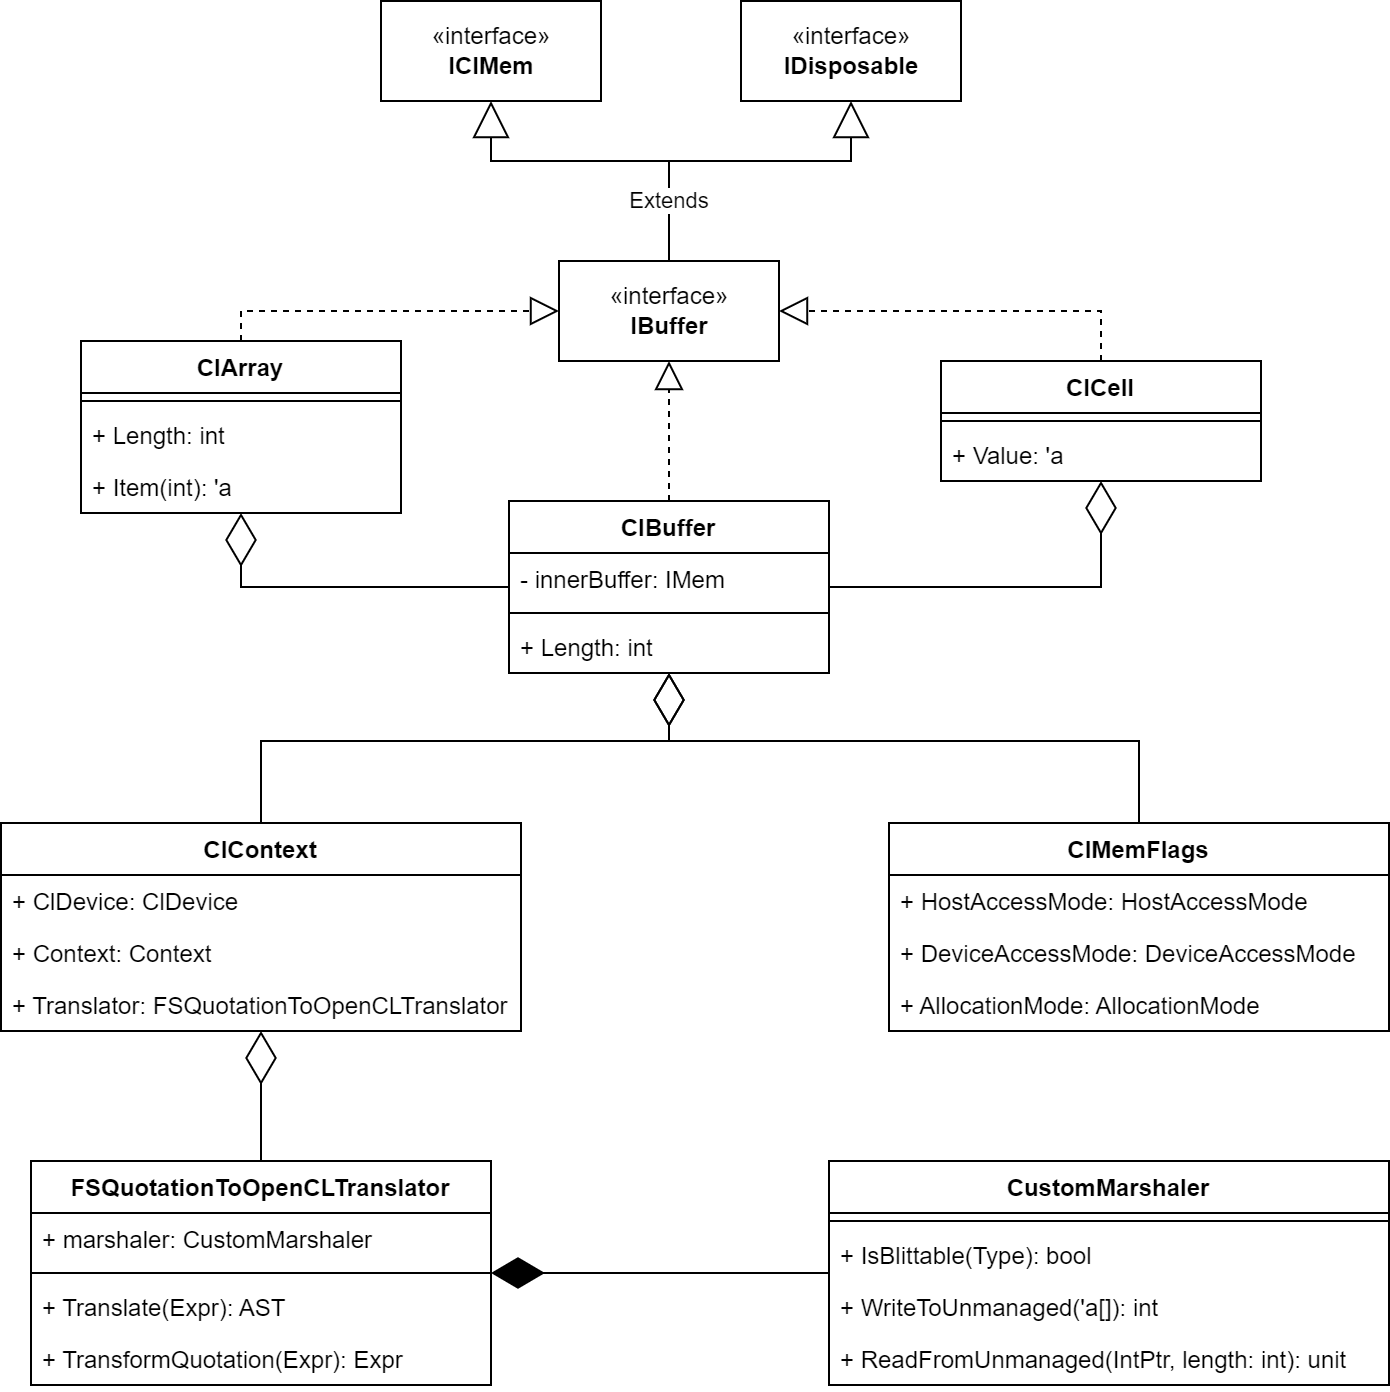
\includegraphics[scale=0.3]{pictures/Mem (1).png}
\caption{Иерархия абстракций в модели управления памятью}
\label{fig:mem}
\end{figure}

\begin{figure}
\centering
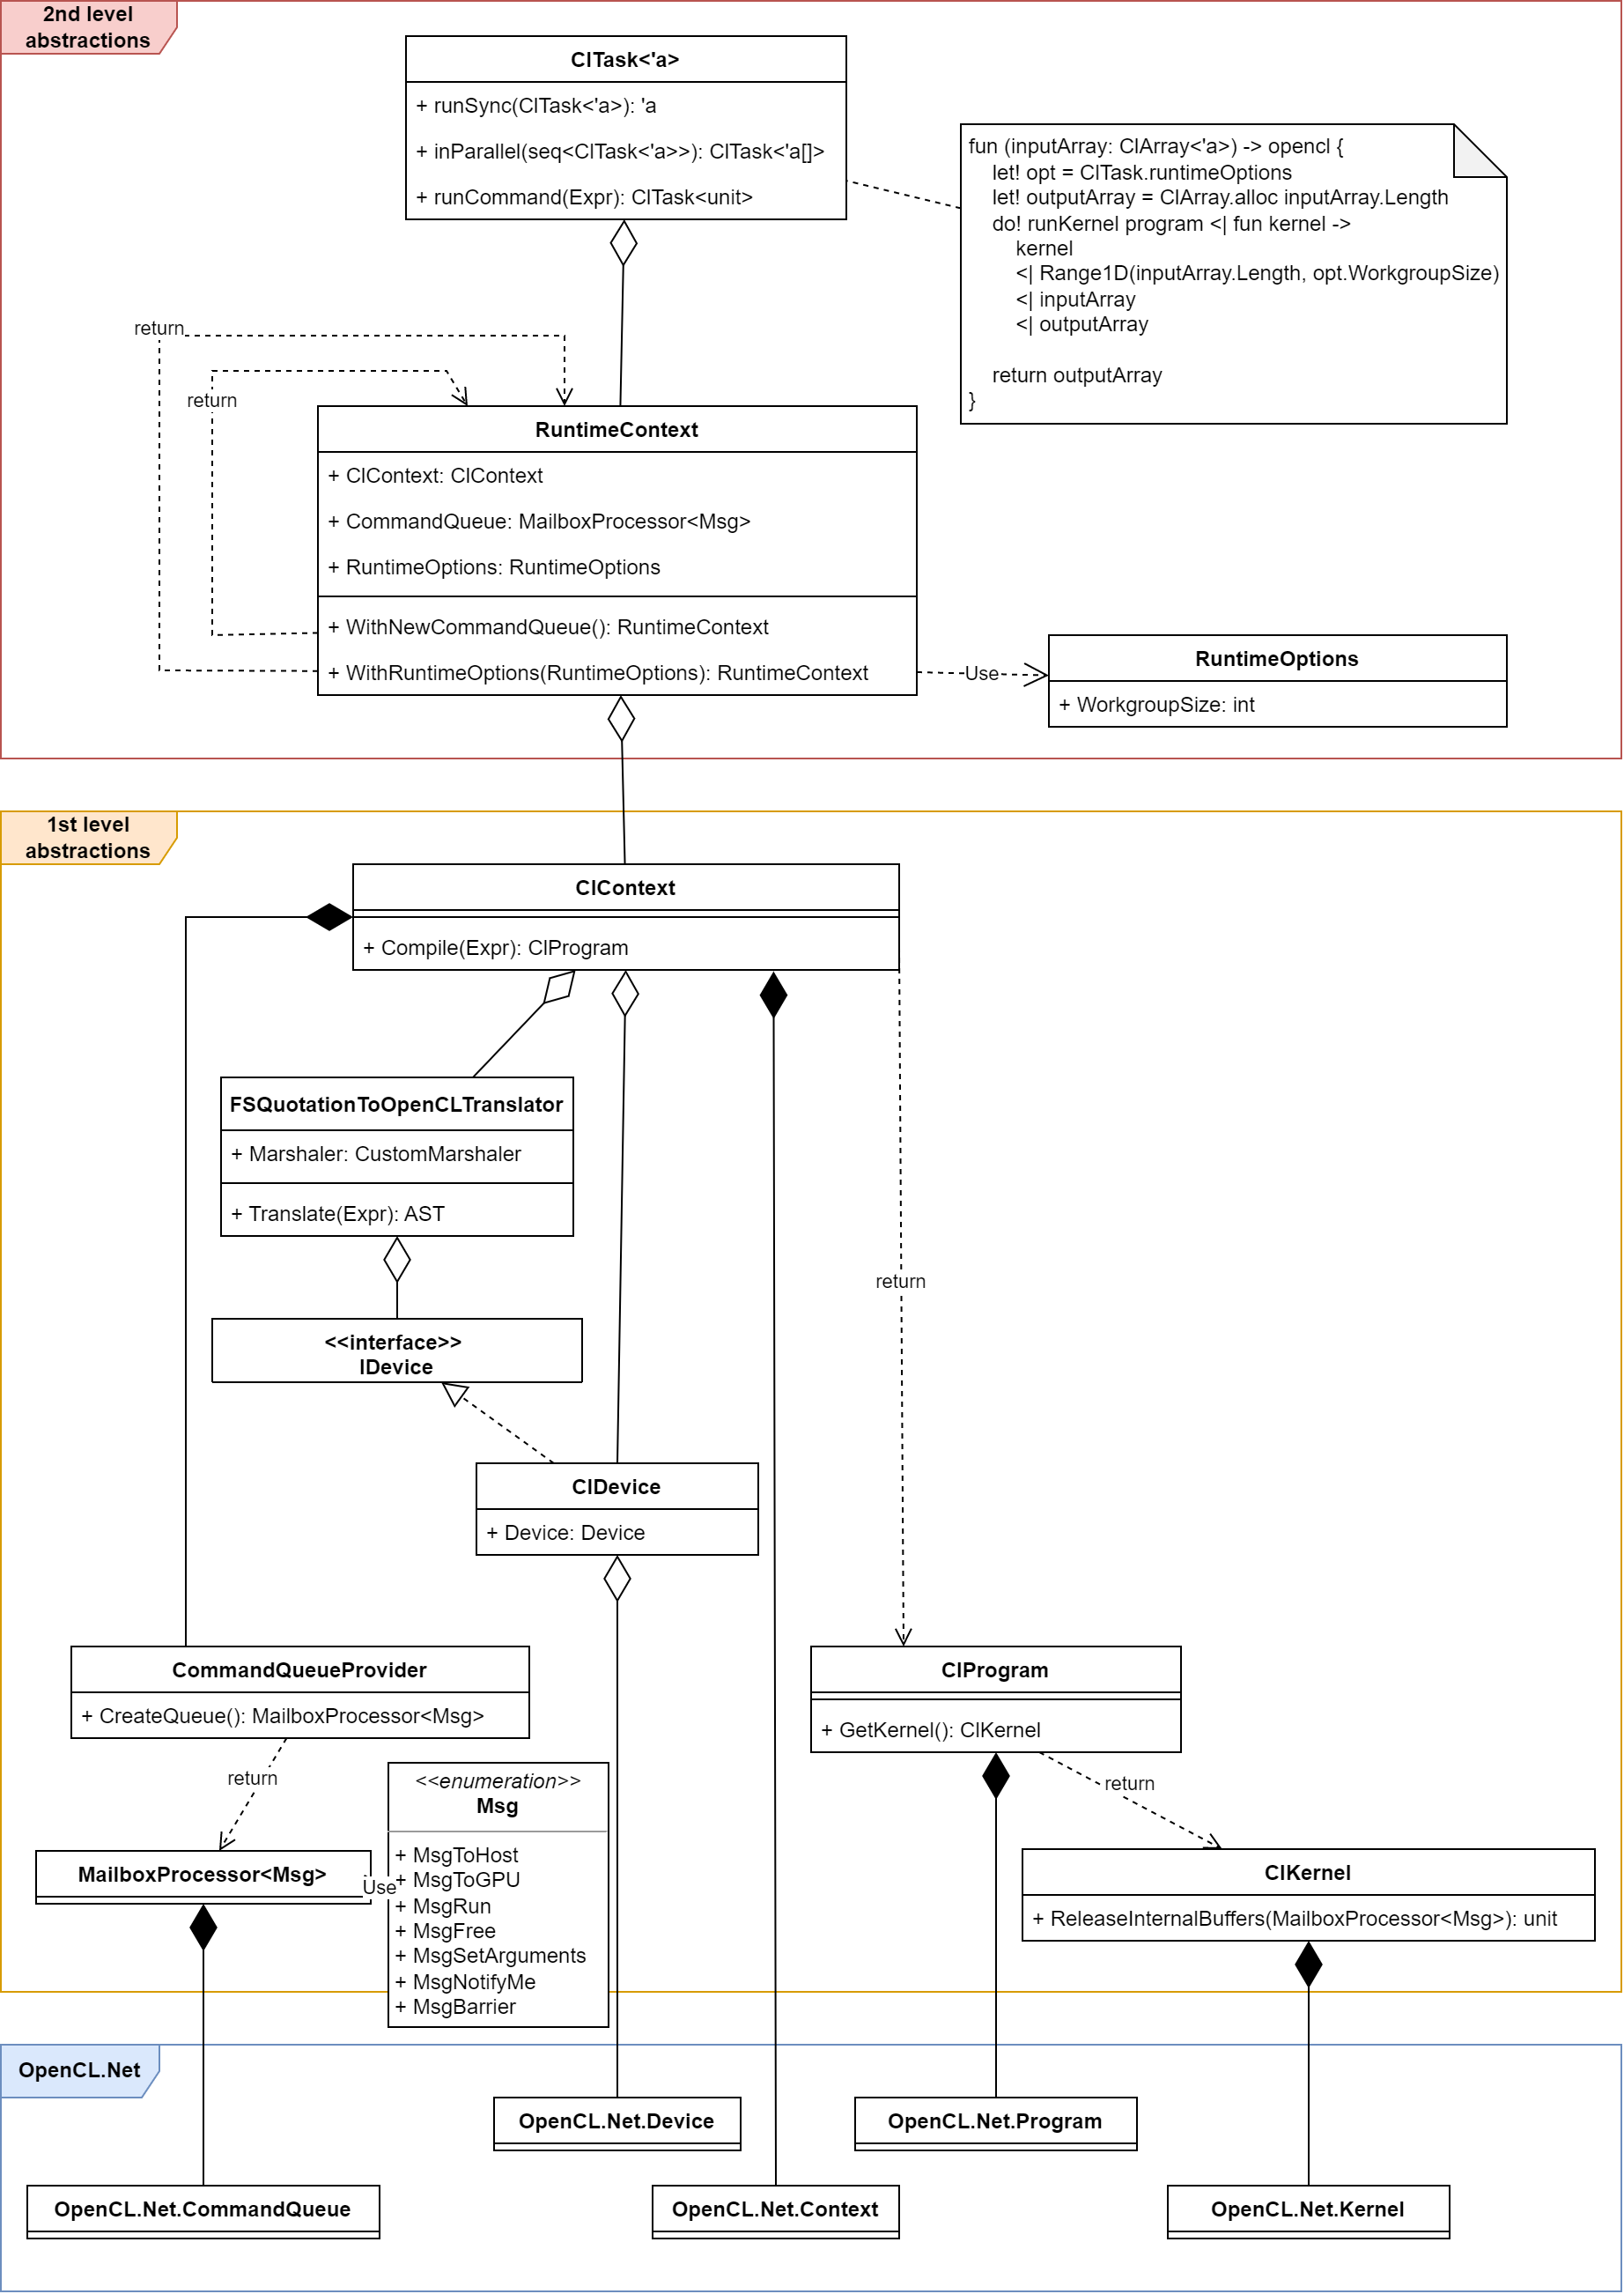
\includegraphics[scale=0.25]{pictures/class.png}
\caption{Общая архитектура решения}
\label{fig:ar}
\end{figure}